\chapter{Teoria}%
\label{ch:teoria}

\section{Stereoanalyysi}

Stereoanalyysi kuvankäsittelyssä tarkoitetta kahdesta samasta kohteesta otetusta kuvasta olevien yhtenäisyyksillä syvyyden analysointia.
Vaikka näitä tekniikoita voi soveltaa mihin tahansa kuviin jotka ovat samasta kohteesta \cite{SumiYasushi20023ORi},
tässä yhteydessä käytämme kuvia,
jotka ovat otettu samasta perspektiivistä siten että kuvat ovat horisontaalisesti vierekkäin.
Jos tiedetään kameroiden suhteelliset sijainnit tai jonkin pisteen etäisyys kamerasta voidaan myös kuvasta arvioida absoluuttinen etäisyys kameraan. 

\begin{figure}[h]
\centering
\pdftooltip{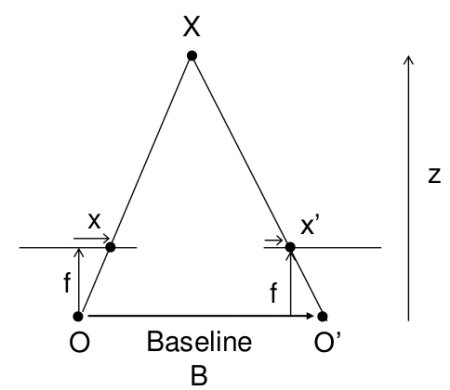
\includegraphics[width=\textwidth]{figures/stereo_depth.jpg}}{Stereo depth}
\caption{Stereosyvyyden arviointi}
\label{fig:stereo}
\end{figure}
    
Kun stereoparia analysoidaan ja tunnistetaan korreloiva piste molemmista kuvista,
voidaan laskea kuvien välinen dispariteetti Kuva \ref{fig:stereo}
Tämä tarkoittaa käytännöstä muutosta pisteen sijainnissa kuvien välillä.
Periaatteessa vastaavat pisteet voivat sijaita missä tahansa kuvassa.
Kuitenkin tässä tapauksessa jossa kuvat ovat tietyssä suhteessa toisiinsa,
voidaan olettaa stereoparin löytyvän x-akselilta tai ainakin melko läheltä sitä.
Jos näin ei olisi jouduttaisiin kuvan jokaista pistettä vertaamaan jokaiseen pisteeseen toisessa kuvassa.
Tämä tapa tulee nopeasti laskennallisesti hyvin kalliiksi.
Jos verrattava alue on myös hyvin pieni todennäköisyys tunnistaa useita samankaltaisia alueita kasvaa.
Jos alue on suuri tai vertailu suoritetaan liian tarkasti,
kasvaa todennäköisyys että vaihtunut kuvakulma on niin erilainen että sitä ei tunnisteta.
Tästä johtuen tämän ongelman ratkaisuun on kehitetty monia erilaisia tapoja.


\subsection{SGM - Semi Global Matching}

Jotta stereoanalyysi on mahdollista,
tulee kuvasta tunnistaa samat kohteet.
Yksi tapa tehdä tämä on Hircmullerin SGM tekniikalla \cite{hirschmuller2005babel}.
Tämä tekniikka ottaa huomioon pikselin ja sen ympäröivien pikselien arvot etsiessään toisesta kuvasta vastaavaa arvoa. Tämä haku voidaan tehdä kaavalla.

\begin{equation}\label{yht:SGM}
    E(d) = \sum_{p} D(p, d_p) + \sum_{q \in \mathcal{N}} R(p, d_p, q, d_q)
\end{equation}

Funktiossa \(D(p, d_p)\) summafunktio käy läpi kaikki kuvan pikselit ja vertaa niitä vertailupikseliin.
Tämä antaa perusarvon yksittäisen pikselin samankaltaisuudelle.

Tämän jälkeen pikselin ympäröiviä pikseleitä verrataan toisiinsa \(R(p, d_p, q, d_q)\).
Koska samaa asiaa ympäröivien pikselien tulisi olla samankaltaisia molemmissa kuvissa,
vaikka ne onkin kuvattu hieman eri asennosta, voidaan tämän avulla arvioida onko kyseessä sama piste.

Tämän algoritmin toteuttaa pythonin opencv kirjaston SGBM \cite{opencvsgbm},
jota muokattu alkuperäiseen toteuytukseen verrattuna käymään läpi pikselijoukkoja, eikä yksittäisiä pikseleitä.
Tämä nopeuttaa prosessointia huomattavasti \cite{MemoryEfficientSGM}.

\section{Neuroverkot} 

Tämän työn lopputulos on neuroverkko.
neuroverkko on yleisesti kuva-analyysiin sekä muuhun koneoppimiseen käytettävä tekniikka.
Sen toiminta perustuu neuroneihin joita järjestetään verkkomaiseen rakenteeseen useisiin eri kerroksiin.
Sen lähtökohta on ihmisaivojen toiminnan matkiminen joka on nykyisen koneoppimistekniikan perusta \cite{PhamTrungQuang2023EotH}.


\begin{equation}\label{yht:neuroni}
    a = \sigma\left(\sum_i w_i x_i + b\right)
\end{equation}

Yllä on neuroverkoissa käytettävän neuronin matemaattinen kaava,
se tuottaa ulostulonaan arvon \(a\) saamiensa syötteiden perusteella.
\(x_i\) on neuronin saama syöte.
\(w_i\) on neuronille annettu painoarvo.
\(b\) on neuronin harha arvo. \(\sigma\) on funktio joka muuttaa neuronin saavan arvon välille 0,1.


Neuroverkko on siis vain joukko yksinkertaisia matemaattisia funktioita,
joiden toimintaa muokkaamalla pyritään saamaan haluttu lopputulos.
Jotta lopputulos on koskaan haluttu pitää tätä koulutusprosessia kuitenkin valvoa.


Kun näitä neuroneita asetetaan eri kerroksiin siten että verkon sisääntulo on esimerkiksi valokuvan kokoinen, 
ja ulostulo on yhen neuronin ulostulo, 
voidaan verkolle syöttää kuvia esimerkiksi kissoista ja koirista.
Kun näille kuville annetaan arvot 0 ja 1 kuvan aiheen mukaan, voidaan verkko kouluttaa tunnistamaan kissoja ja koiria.
Koulutuksen aikana verkko muuttaa arvojaan \(w_i\) ja \(b\).
Nämä arvot se saa yrittämällä erilaisia arvoja neuroneille.
Kun verkkoa tämän jälkeen testataan on voidaan saaduista lopputuloksista valita paras.
Tämän jälkeen tätä lopputulosta voidaan lähteä parantelemaan, testaamalla toimiiko suuremmat vai pienemmät arvot paremmin.
Kun näitä kahta arvoa eri neuroneilla muutetaan voidaan saada paremmin toimiva neuroverkko.
Tarpeeksi monen yrityksen jälkeen, saadaan siis todennäköisesti verkko joka tunnistaa onko kuvassa todennäköisemmin kissa vai koira

Tätä satunnaisuutta pyritään siis parantamaan ohjaamalla verkon koulutusta.
Tämä tapahtuu tappiofunktion (loss function) sekä takaisinvirtausalgoritmin (backpopagation algorithm) avulla.

Tappiofunktion tehtävä on kertoa kuinka paljon saatu tulos eroaa halutusta.
Esimerkkitapauksessamme tämä käytännössä testaa, verkon lopputuloksen ja palauttaa kuinka monta arvausta verkko sai oikein,
tämä käytännössä katsoisi onko verkolle annetun kissa kuvan ulostulon arvo mikä sen pitäisi olla.
Virheen tunnistus ei kuitenkaan ole aina yhtä yksinkertaista, tämän työn lopputulos on verkko joka yrittää luoda kuvasta 3d pistekartan.
Siinä tapauksessa siis neliösumma tai jokin muu tapa virheen tunnistamiseen olisi parempi.
Kun virhe on tunnistettu verkkoa muokataan takaisinvirtaus algoritmin perusteella.
Näihin algoritmeihin ei ole yhtä parasta ratkaisua, vaan eri verkkojen ja käyttökohteiden tapauksessa eri algoritmit voivat tuoda hyvin erilaisia tuloksia.

\section{Semantic segmentation}

Semantic segmentation eli kuvan segmentointi on yleinen käyttökohde neuroverkoille.
Sen avulla on helppo tehdä käytettäviä ja helposti hyödynnettäviä malleja.
Ja se on hyvä esimerkki ongelmasta jolle on helppo tehdä koulutusdataa, mutta hankala luoda ohjelmallista toteutusta saman lopputuloksen saamiseksi.
Esimerkkejä käytöstä on esimerkiksi automatisoidussa liikenteessä esteiden tunnistuksessa Kuva \ref{fig:labels}.

\begin{figure}[h]
\centering
\pdftooltip{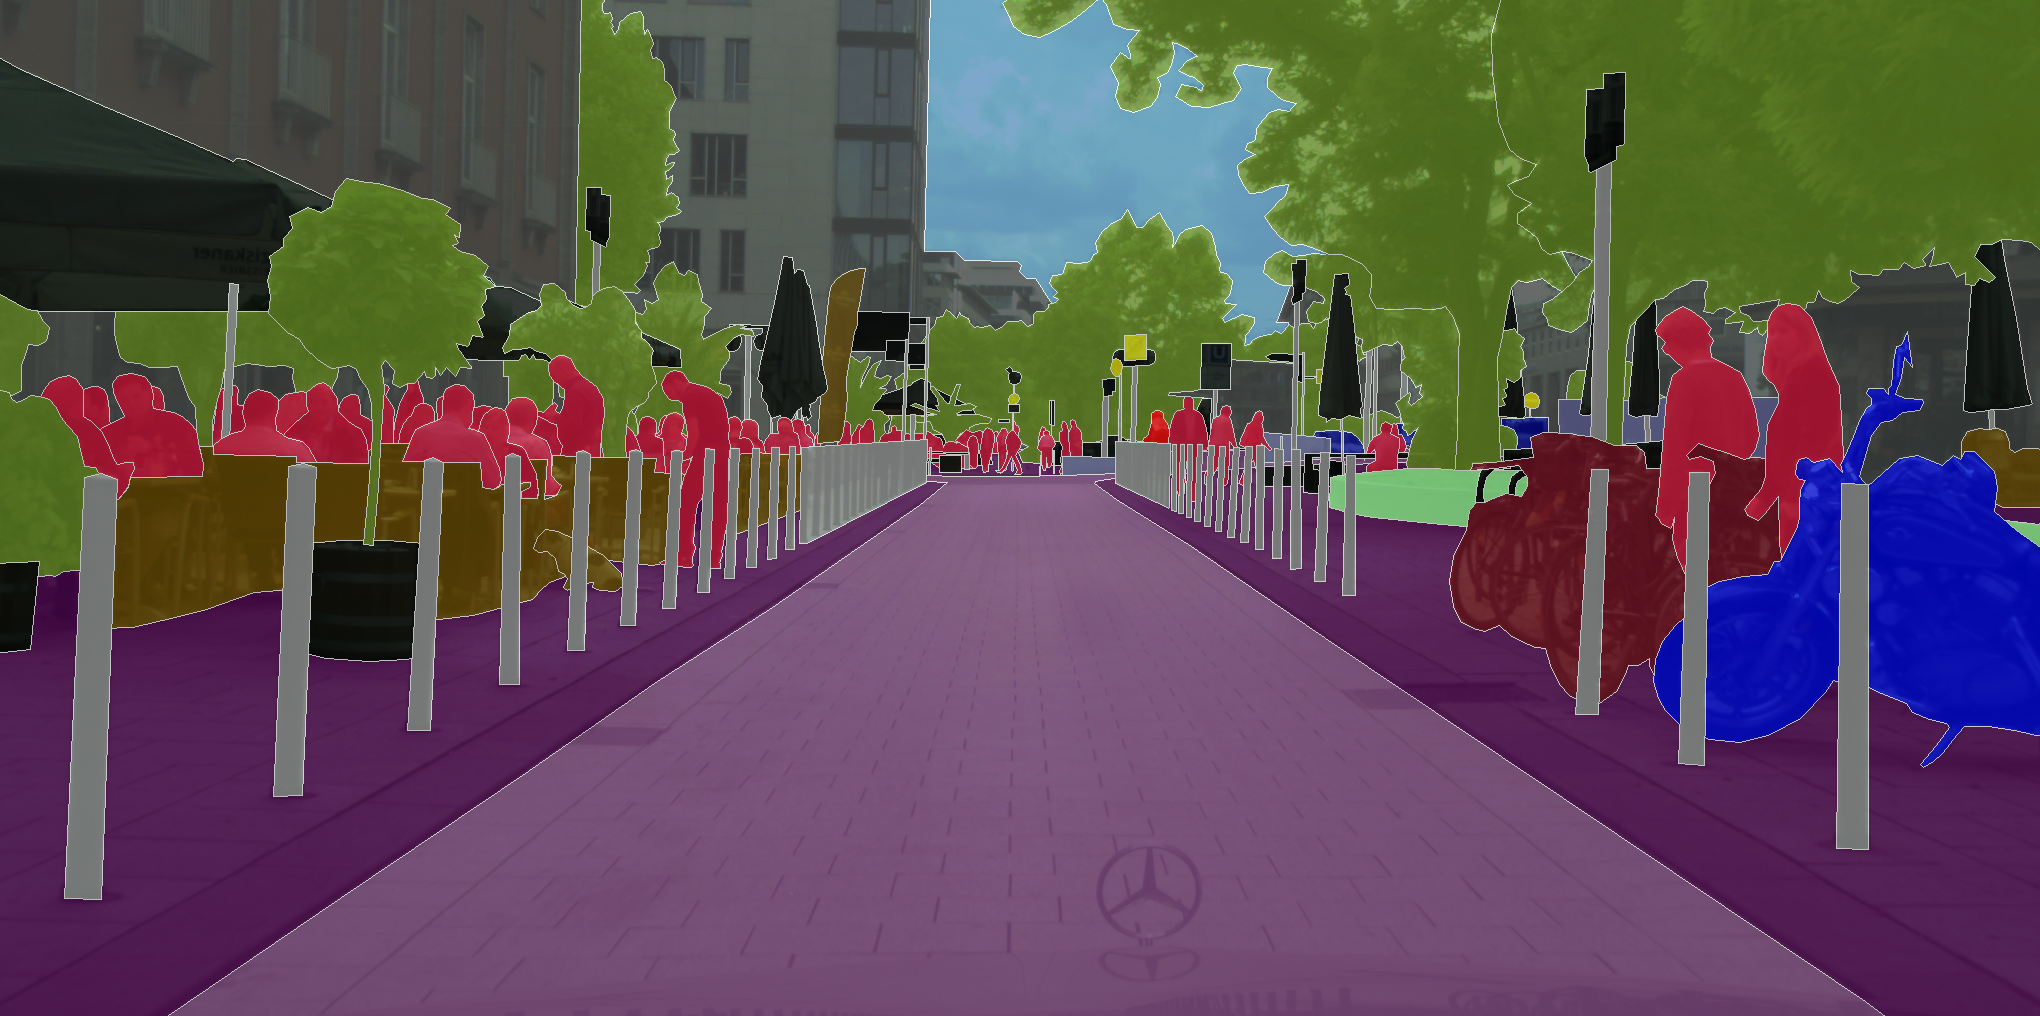
\includegraphics[width=\textwidth]{figures/stuttgart03.png}}{Cityscapes esimerkki kuva stuttgart03}
\caption[Tämä on lyhyt kuvateksti.]{Cityscapes datestin esimerkki segmentointi dataa, jossa kaupunkinäkymän erilaiset tunnistattavat kohteet on merkitty eri väreillä.}
\label{fig:labels}
\end{figure}

Tätä teknologiaa voidaan soveltaa useiden eri tunnistusongelmien ratkaisuun.
Koulutusdatasta riippuen malli voiddaan kouluttaa minkä tahansa kuvassa näkyvän kohteen tunnistukseen.
Samaa teknologiaa käytetään teollisissa sovellutuksissa laadunvalvonnassa,
sekä lääketieteessä erilaisten skannausten analysoinnissa \cite{NagalakshmiT2022BCSS}.
Mallin voi kouluttaa tunnistamaan useita tai vain yhtä asiaa riippuen käyttökohteesta.
Toisin kuin perinteinen tunnistusmalli, joka tunnista yleensä vain mitä kuvassa on,
segmnetaatiomalli antaa joka pikselille arvon jonka perusteella lopputuloksesta voidaan nähdä, mitä eri kohdissa kuvaa on.
Jotta samanlainen lopputulos saataisiin kohteentunnistusmallilla, pitäisi kuvaa käydä läpi pienemmissä lohkoissa jotta rajat löytyisivät.
Kohteen tunnistusta voisi myös hyödyntää eri kohteiden etäisyyden arviointiin, jota voisi hyödyntää niiden takana olevan syvyyden arvioimiseen \cite{ShiZhou2023VRBo}.

Segmentointimallin kouluttaminen ja datasetin käsittely on hieman haastavampaa kuin kohteentunnistusmallin.
Jotta mallin voi kouluttaa tunnistamaan asiat pikselitasolla, on myös opetusdatan oltava pikselitasolla määriteltyä. 
Myöskin datan koulutuksessa käytettävä tappiofunktion määrittely hieman hankaloituu.
Mallin koulutuksessa pitää käyttää jotain muuta tapaa tunnistaa sen onnistuminen, kuin vain ”onko kyseessä auto”.

Yksi segmentointimallin koulutuksessa käytettävä tappion laskutapa, 
jota myös tässä työssä käytetään, on ristientropian virhefunktio (Cross Entropy Loss) \cite{CrossEntropyLoss}. 

Ristientoripa virhefunktio vertaa mallin tuottamia toednnäköisyyksiä oikeaan malliin. 
Sille lasketaan virhe ottamalla negatiivinen logaritmi oikeaan luokkaan liittyvästä todennäköisyydestä ja lisäämällä sen arvo kaikkien havaintojen yli.
Tämä siis tarkoittee, että mallin ennustaman todennäköisyyden ja todellisen luokan välille lasketaan epävarmuus jonka avulla mallia voidaan ohjata oikeaan suuntaan.
Mitä enemmän alueet osuvat oikeaan, sitä pienemmäksi mallin virhe laskee.

\section{Syvyyskartta}

Tämän työn haluttu lopputulos on syvyyskartta \cite{IkeuchiKatsushi1987DaDM}.
Syvyyskartta on yksinkertainen kuvan kaltainen esitystapa, jossa eri syvyyksillä on eri numeerinen arvo.
Se voidaan näyttää esimerkiksi siten että kauempana kamerasta oleva kohde on tummemmalla värillä \ref{fig:depth}.
Tärkeä ero 3d-malliin sekä syvyyskartan välillä on datan perspektiivi.
Syvyyskartassa ei ole tietoa kohteiden takana olevasta tilasta, joten sitä voi tarkastella vain sen perspektiivistä, eikä näin ollen "pyörittää" yhtä vapaasti kuin 3d mallia.


\begin{figure}[h]
\centering
\pdftooltip{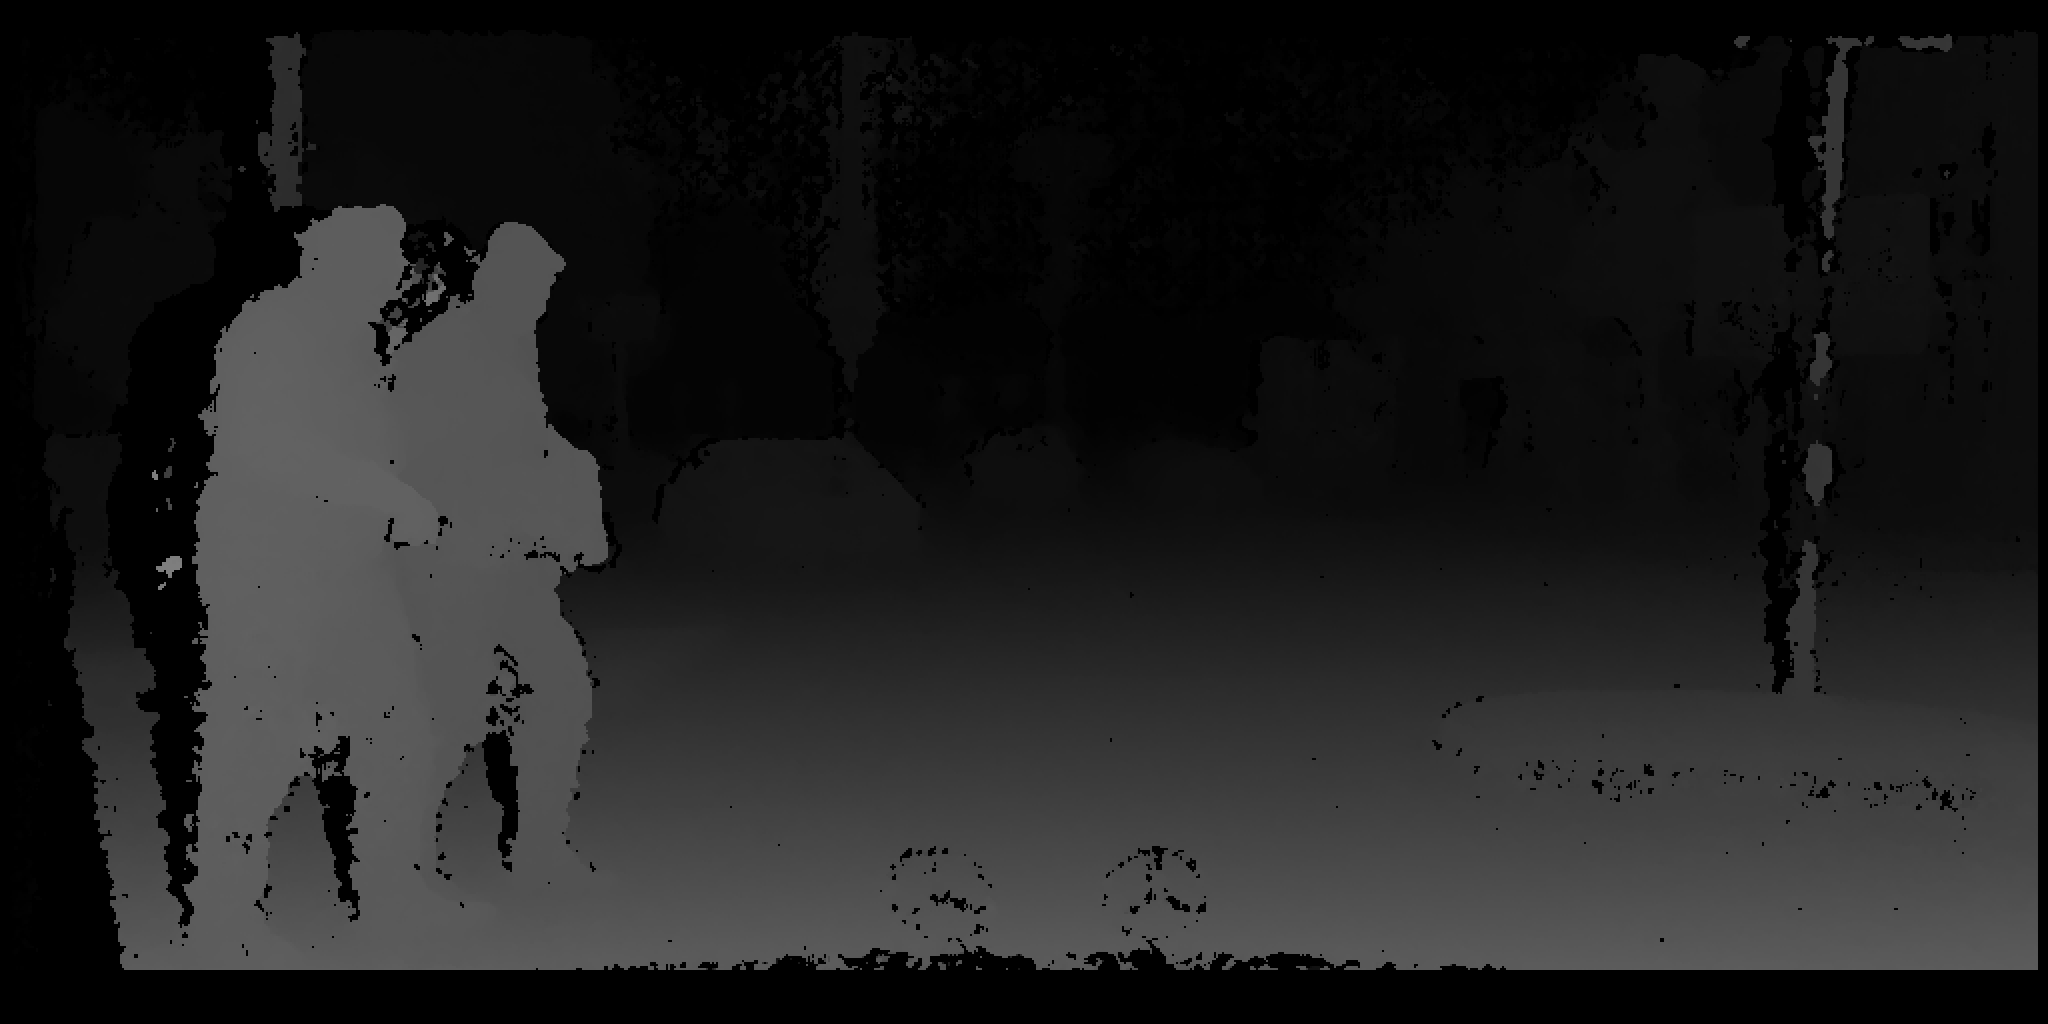
\includegraphics[width=\textwidth]{figures/leverkusen_000024_000019_disparity.png}}{Cityscapes esimerkki kuva leverkusen_000024_000019_disparity}
\caption[Tämä on lyhyt kuvateksti.]{Citysscapes datasetin syvyysdata esimerkki.}
\label{fig:depth}
\end{figure}
